\chapter{Pseudohalide complexes}
\section{Chemical properties}
Pseudohalogenes are polyatomic molecules posessing properties similar to halogenes and are therefore among the group of pseudoelements. These chemical properties are reactivity, charge and binding behavior. They can be used as substitutions for halogenes in all kinds of chemical  compounds. Pseudohalides, the ionic form of pseudohalogenes, are used as ligands in coordination complexes. Cyanide, cyanate, thiocyanate, azides and rhodanides are well known pseudohalides. The chemical properties and their behavior are identical to halide ions. The internal double or triple bonds that are often present do not affect their chemical behavior. They form strong acids (HX) and  react with metals to form compounds like MX. \cite{holub}


\section{Azide complexes}

Azide (\ce{N_3^-}) is the salt of hydrazoic acid. \ce{HN_3} is a weak base (pk$_a$ of 4.75) and is highly explosive in its waterfree form.
Hydrazoic acid and azides are highly toxic and should be handled with care. The linear molecule N$_3^-$ has three possible resonance structures: \\
\ce{ ^{-}N = N^{+}= N^{-} <=> N# N^+ - N^{2-} <=> ^{2-}N - N^+ # N}\\
Azide can be organised in two types: inorganic  (e.g. NaN$_3$) and organic azides (e.g. TosN$_3$). \cite{holub}
 Furthermore, azides can be subdivided in more types according to their bonding character \cite{mueller}: Ionic azides, molecular azides and coordinative azides.\\
Azides are used for technical applications such as explosives (\ce{Pb(N3)2}), airbags or pharmacy. Fig. \ref{fig:az} depicts bridging modes of azides. 
\begin{figure}[htpb!]
\centering
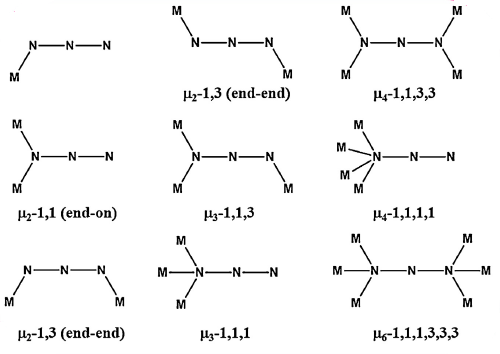
\includegraphics[scale=1]{figures/azidescheme.png}
\caption{Structures of published azide complexes \cite{han2015}}
\label{fig:az}
\end{figure}

\section{Rhodanide and cyanate complexes}
Thiocyanate (alternate name rhodanide) is the conjugate base of thiocyanic acid. Common derivatives are KSCN and NaSCN. Rhodanite is an analogue of the cyanate ion (\ce{OCN^-}). The name rhodanide means rose in greek  and comes from the red colour of its iron complexes. If the metal or the organic group is attached to the S (\ce{R-S-C#N}) the compound is called thiocyanate and if it is bonded to the N-atom (\ce{R-N=C=S}) its name is isothiocyanate. \cite{guy1977} Two equivalent resonance structures exist:\\
\ce{S=C=N^- <=> ^-S-C#N} \\
As a result thiocyanate is an ambidentate ligand, meaning that both ends (S or N) can act nucleophilic. In fig. \ref{fig:ocnscn} I-VI are listed the known bonding types. Hard acids form N-bonded isothiocyanate complexes and soft acids form S-bonded thiocyanate complexes.\cite{holub}  \\
\begin{figure}[htpb!]
\centering
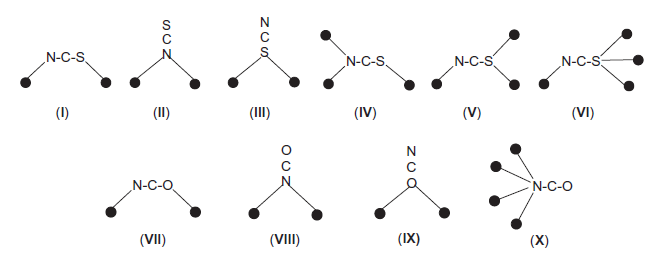
\includegraphics[width=1\textwidth]{figures/schemeocnscn.png}
\caption{Some thiocyanate and cyanate coordination bridging modes. Points represent metallatoms. \cite{fam}}
\label{fig:ocnscn}
\end{figure}

Cyanate's chemical structure is [OCN]$^-$ or [NCO]$^-$. It has similar properties to thiocyanate. In figure \ref{fig:ocnscn} (VII) to (X) the different bonding types are shown.  If the metal or the organic group is attached to the O (\ce{R-O-C#N}) the compound is called cyanate and if it is bonded to the N-atom (\ce{R-N=C=O}) its name is isocyanate. \cite{holub}


\section{Dicyanamide complexes}




The molecular formula for dicyanamide is \ce{C_2N_3^-}. It is composed of two cyanide groups that are bound to a central nitrogen anion. It can be used as a counterion in organic and inorganic salts and as reactant for the synthesis of covalent organic structures.
Another use would be the synthesis of pseudohalide complexes. The metal  can bind on the middle and end nitrogen atoms of the dicyanamide. Therefore there are a lot of combinations how the metals can be bound to a single dicyanamide. \cite{holub} In fig. \ref{fig:syndca} there are examples of structures of published dca complexes. Fig. \ref{fig:nosyndca} contains structures which have not been synthesized yet but are also possible. 

\begin{figure}[h!]
\centering
\subfigure[0-1-0]{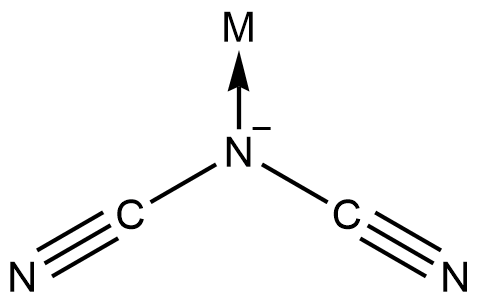
\includegraphics[scale=0.35]{figures/dca0-1-0.png}}
\quad
\subfigure[1-0-0]{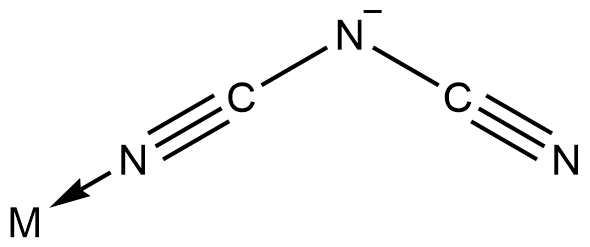
\includegraphics[scale=0.35]{figures/dca1-0-0.png}}
\subfigure[1-0-1]{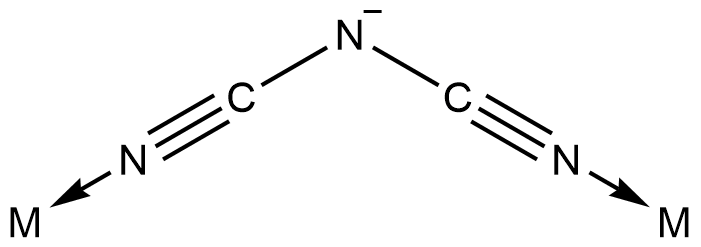
\includegraphics[scale=0.35]{figures/dca1-0-1.png}}
\quad
\subfigure[1-1-0]{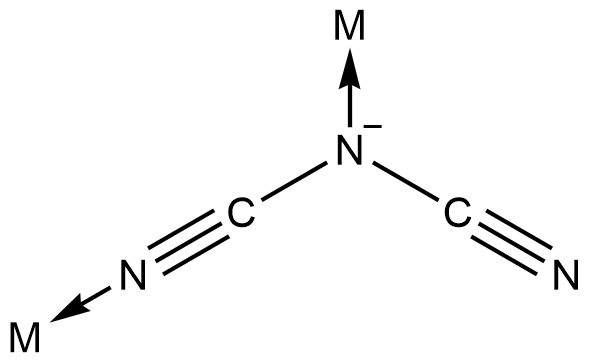
\includegraphics[scale=0.35]{figures/dca1-1-0.png}}
\subfigure[1-1-1]{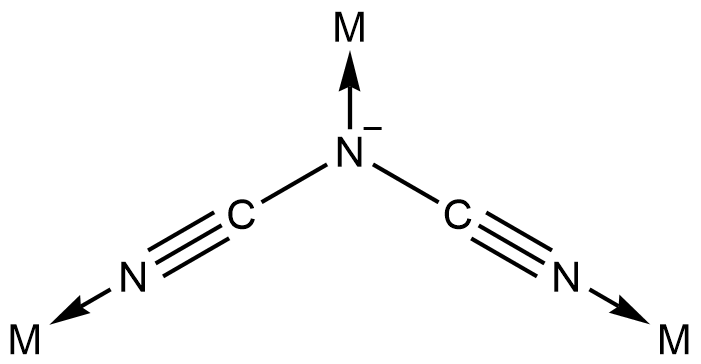
\includegraphics[scale=0.35]{figures/dca1-1-1.png}}
\quad
\subfigure[2-0-0]{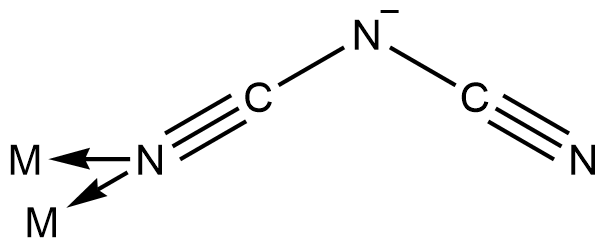
\includegraphics[scale=0.35]{figures/dca2-0-0.png}}
\subfigure[2-0-1]{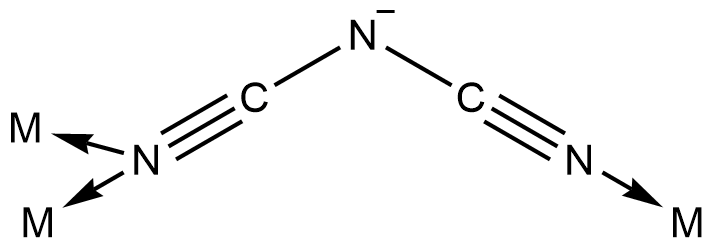
\includegraphics[scale=0.35]{figures/dca2-0-1.png}}
\quad
\subfigure[2-0-2]{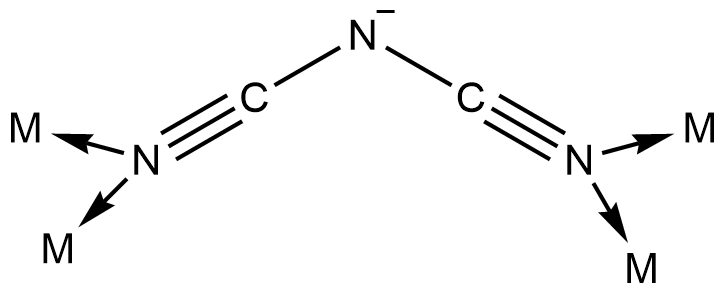
\includegraphics[scale=0.35]{figures/dca2-0-2.png}}

\caption{Structures of published dca complexes in the CCDC \cite{ccdc}}
\label{fig:syndca}
\end{figure}


\begin{figure}[h!]
\centering
\subfigure[2-1-0]{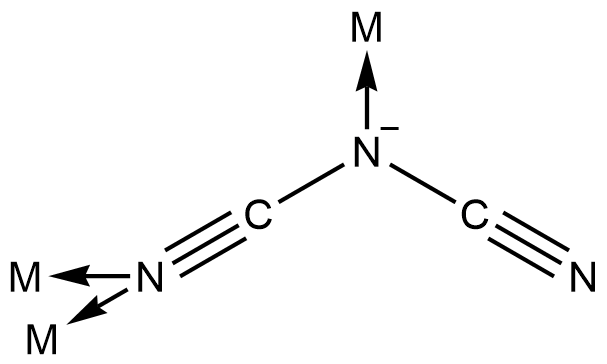
\includegraphics[scale=0.35]{figures/dca2-1-0.png}}
\quad
\subfigure[3-0-0]{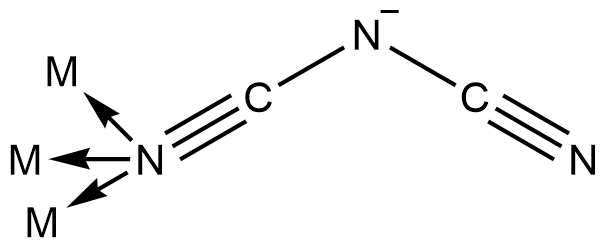
\includegraphics[scale=0.35]{figures/dca3-0-0.png}}
\subfigure[3-0-2]{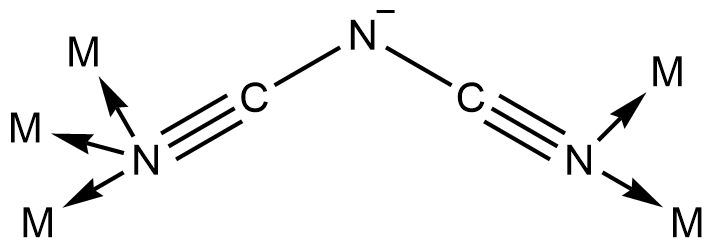
\includegraphics[scale=0.35]{figures/dca3-0-2.png}}
\quad
\subfigure[3-0-3]{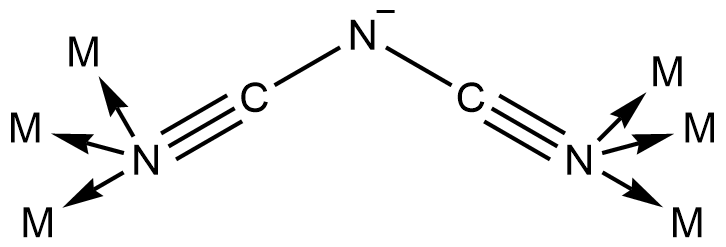
\includegraphics[scale=0.35]{figures/dca3-0-3.png}}
\subfigure[4-0-0]{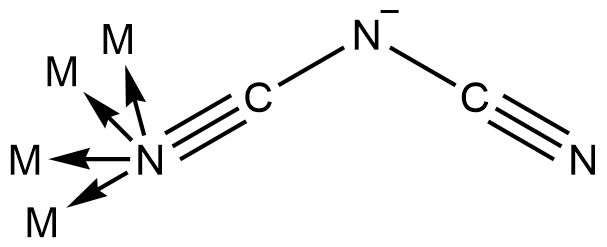
\includegraphics[scale=0.35]{figures/dca4-0-0.png}}


\caption{Structures of possible dca complexes which are not  published yet}
\label{fig:nosyndca}
\end{figure}








